\documentclass[11pt]{charter}

% El títulos de la memoria, se usa en la carátula y se puede usar el cualquier lugar del documento con el comando \ttitle
\titulo{Estimación de la captura realizada en buques pesqueros mediante visión artificial} 

% Nombre del posgrado, se usa en la carátula y se puede usar el cualquier lugar del documento con el comando \degreename
%\posgrado{Carrera de Especialización en Sistemas Embebidos} 
%\posgrado{Carrera de Especialización en Inteligencia  de las Cosas} 
\posgrado{Carrera de Especialización en Inteligencia Artificial}
%\posgrado{Maestría en Sistemas Embebidos} 
%\posgrado{Maestría en Internet de las cosas}

% Tu nombre, se puede usar el cualquier lugar del documento con el comando \authorname
\autor{Lic. Nicolás Eduardo Horro} 

% El nombre del director y co-director, se puede usar el cualquier lugar del documento con el comando \supname y \cosupname y \pertesupname y \pertecosupname
\director{PhD. Félix Ramón Rojo}
\pertenenciaDirector{INVAP S.E.} 
% FIXME:NO IMPLEMENTADO EL CODIRECTOR ni su pertenencia
%\codirector{} % si queda vacio no se deberíá incluir 
%\pertenenciaCoDirector{}

% Nombre del cliente, quien va a aprobar los resultados del proyecto, se puede usar con el comando \clientename y \empclientename
\cliente{Dr. Jorge Omar Lugo}
\empresaCliente{INVAP S.E.}

% Nombre y pertenencia de los jurados, se pueden usar el cualquier lugar del documento con el comando \jurunoname, \jurdosname y \jurtresname y \perteunoname, \pertedosname y \pertetresname.
\juradoUno{Nombre y Apellido (1)}
\pertenenciaJurUno{pertenencia (1)} 
\juradoDos{Nombre y Apellido (2)}
\pertenenciaJurDos{pertenencia (2)}
\juradoTres{Nombre y Apellido (3)}
\pertenenciaJurTres{pertenencia (3)}

\fechaINICIO{05 de marzo de 2021}		%Fecha de inicio de la cursada de GdP \fechaInicioName
\fechaFINALPlanificacion{23 de abril de 2021} 	%Fecha de final de cursada de GdP
\fechaFINALTrabajo{10 de diciembre de 2021}		%Fecha de defensa pública del trabajo final


\begin{document}

\maketitle
\thispagestyle{empty}
\pagebreak


\thispagestyle{empty}
{\setlength{\parskip}{0pt}
\tableofcontents{}
}
\pagebreak


\section{Registros de cambios}
\label{sec:registro}


\begin{table}[ht]
\label{tab:registro}
\centering
\begin{tabularx}{\linewidth}{@{}|c|X|c|@{}}
\hline
\rowcolor[HTML]{C0C0C0} 
Revisión & \multicolumn{1}{c|}{\cellcolor[HTML]{C0C0C0}Detalles de los cambios realizados} & Fecha      \\ \hline
1.0      & Creación del documento.                                          & 05/03/2021 \\ \hline
1.1      & Correcciones de primera revisión. Historias de usuario.          & 28/03/2021 \\ \hline
1.2      & Diagramas AoN y Gantt. Matrices RUM y RAM. Presupuesto.          & 01/04/2021 \\ \hline
1.3      & Aplicadas observaciones de última revisión. Se completan secciones 12-17.   & 08/04/2021 \\ \hline
\end{tabularx}
\end{table}

\pagebreak

\section{Acta de constitución del proyecto}
\label{sec:acta}

\begin{flushright}
San Carlos de Bariloche, \fechaInicioName
\end{flushright}

\vspace{2cm}

Por medio de la presente se acuerda con el Lic. \authorname\hspace{1px} que su Trabajo Final de la \degreename\hspace{1px} se titulará ``\ttitle'', consistirá esencialmente en el prototipo preliminar de un sistema para clasificación de capturas y descarte en buques pesqueros que utiliza técnicas de visión por computadora e inteligencia artificial, y tendrá un presupuesto preliminar estimado de 600 hs de trabajo, con fecha de inicio \fechaInicioName\hspace{1px} y fecha de presentación pública \fechaFinalName.

Se adjunta a esta acta la planificación inicial.

\vfill

% Esta parte se construye sola con la información que hayan cargado en el preámbulo del documento y no debe modificarla
\begin{table}[ht]
\centering
\begin{tabular}{ccc}
\begin{tabular}[c]{@{}c@{}}Ariel Lutenberg \\ Director posgrado FIUBA\end{tabular} & \hspace{2cm} & \begin{tabular}[c]{@{}c@{}}\clientename \\ \empclientename \end{tabular} \vspace{2.5cm} \\ 
\multicolumn{3}{c}{\begin{tabular}[c]{@{}c@{}} \supname \\ Director del Trabajo Final\end{tabular}} \vspace{2.5cm} \\
%\begin{tabular}[c]{@{}c@{}}\jurunoname \\ Jurado del Trabajo Final\end{tabular}     &  & \begin{tabular}[c]{@{}c@{}}\jurdosname\\ Jurado del Trabajo Final\end{tabular}  \vspace{2.5cm}  \\
%\multicolumn{3}{c}{\begin{tabular}[c]{@{}c@{}} \jurtresname\\ Jurado del Trabajo Final\end{tabular}} \vspace{.5cm}                                                                     
\end{tabular}
\end{table}

\section{Descripción técnica-conceptual del proyecto a realizar}
\label{sec:descripcion}

El presente proyecto consiste en un prototipo que extiende el Sistema de Monitoreo Electrónico (SME) que incluye sistemas de Circuitos Cerrados de Televisión (CCTV) a bordo de los buques pesqueros mediante el uso Inteligencia Artificial (IA). El objetivo es la automatización del proceso de clasificación y estimación de cantidad de piezas capturadas y descartadas, proceso que actualmente se realiza de manera manual y resulta costoso y propenso a errores. Esta tarea se realiza mediante inspección y es llevada a cabo por operadores humanos.

La figura  \ref{fig:canvas} muestra un diagrama de lienzo (canvas) del modelo de negocio de la solución.

\vspace{25px}

\begin{figure}[htpb]
\centering 
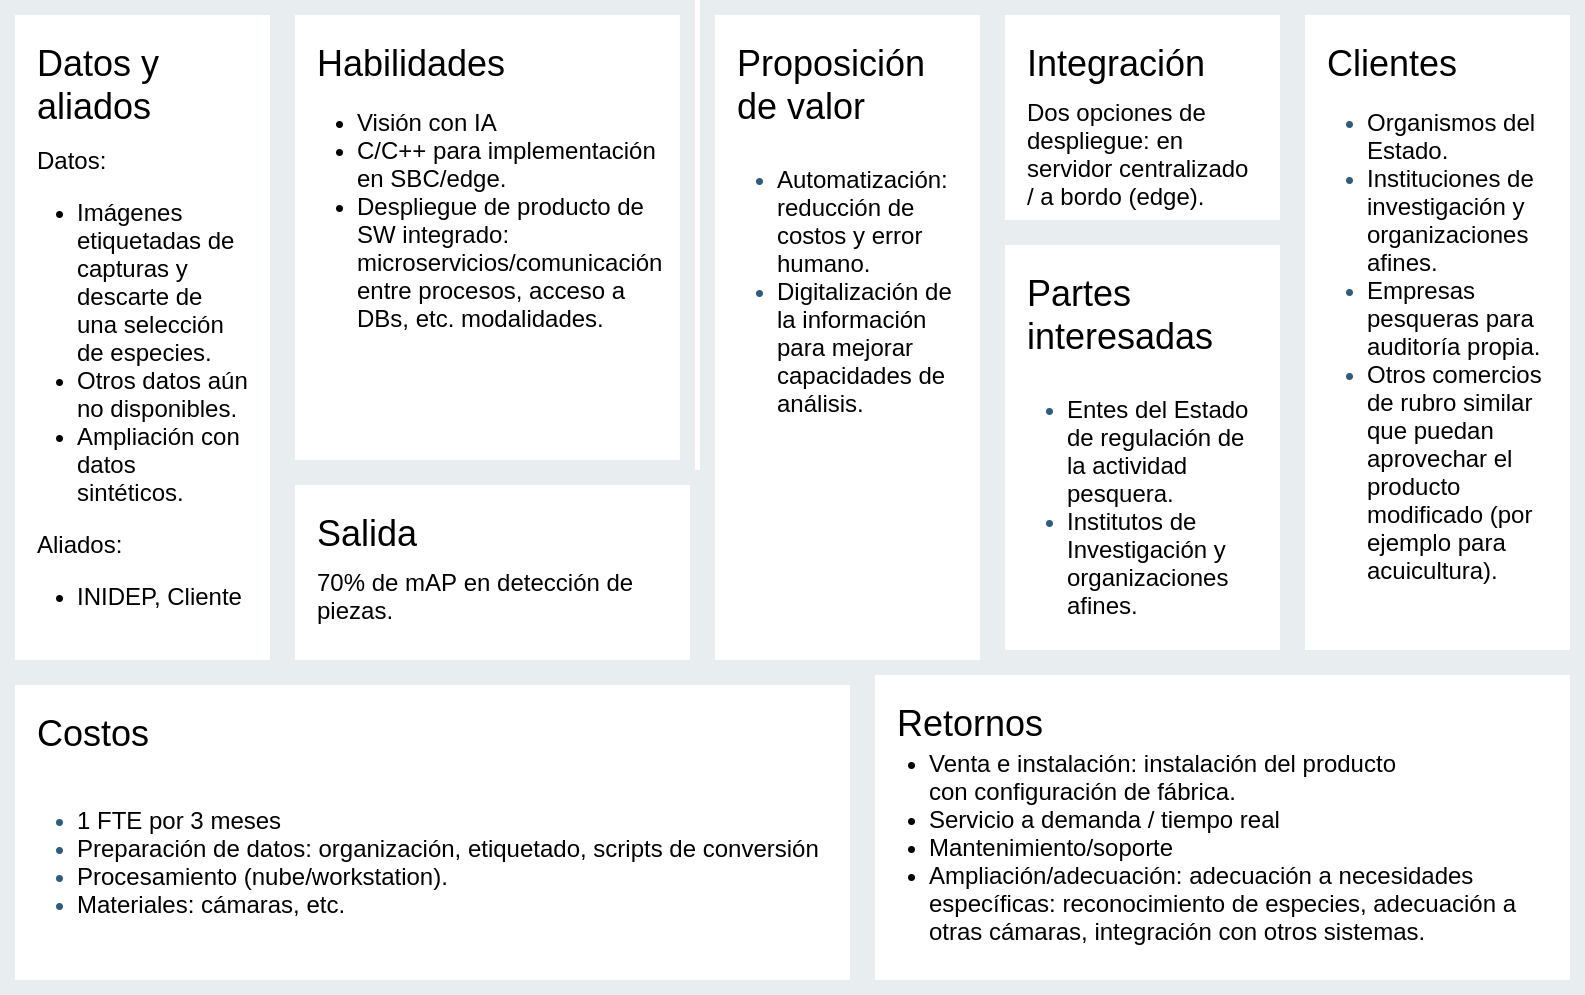
\includegraphics[width=1\textwidth]{./Figuras/canvas.png}
\caption{Diagrama de lienzo (canvas) del modelo de negocio de la solución}
\label{fig:canvas}
\end{figure}

\vspace{25px}

\subsection{Introducción general al tema}

La pesca industrial es un tipo de pesca que tiene como objetivo obtener un gran número de capturas. En Argentina el sector primario pesquero (aquel que se ocupa de la captura) se compone de una flota de buques fresqueros de altura, de costeros grandes y costeros chicos y una flota de buques procesadores. La flota fresquera de altura está conformada por barcos arrastreros con bodegas refrigeradas y cuentan con equipamiento de navegación y detección y utilizan redes de arrastre.

La figura \ref{fig:tipo_embarcaciones} expone un diagrama simplificado de los tipos de embarcaciones y métodos de captura de acuerdo a la profundidad.

\vspace{25px}

\begin{figure}[htpb]
\centering 
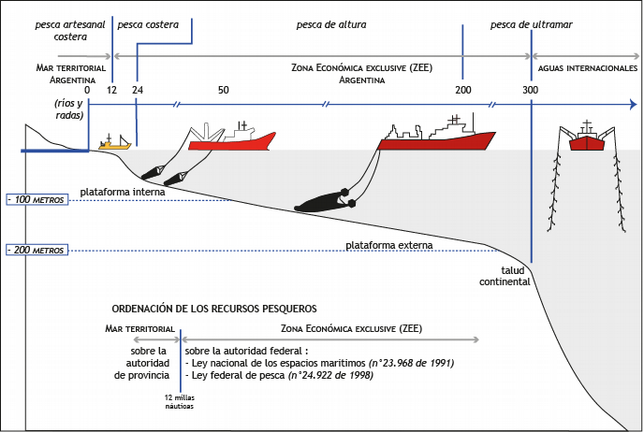
\includegraphics[width=1.\textwidth]{./Figuras/tipo_embarcaciones.png}
\caption{Tipos de embarcaciones según el tipo de pesca}
\label{fig:tipo_embarcaciones}
\end{figure}

\vspace{25px}

A fin de garantizar que la pesca a esta escala sea sostenible, el Consejo Federal Pesquero tiene como funciones el establecimiento de la política pesquera y de la política de investigación pesquera nacional, la planificación del desarrollo pesquero nacional, el establecimiento de la Captura Máxima Permisible (CMP) por especie y las cuotas de captura, así como aprobar los permisos de pesca comercial y experimental y fijar los cánones por el ejercicio de la pesca, entre otros. 
Dado que una pesquería es un sistema complejo de factores interdependientes entre los que se cuentan el estado del recurso biológico, limitaciones sociales e institucionales, condiciones económicas y convicciones culturales, etc., es importante generar información estadística e indicadores que permitan el análisis de la actividad de las pesquerías para poder establecer de manera precisa su marco regulatorio.
El monitoreo y la vigilancia deben permitir conocer las características del esfuerzo en la actividad pesquera y asegurar que las capturan se realicen dentro de los cánones admitidos. Existen también regulaciones que establecen el modo en que debe emplearse la técnica, por ejemplo, exigiendo una permanencia mínima de las redes en el fondo para disminuir la captura incidental de mamíferos marinos.

Tradicionalmente, la principal manera de recopilar información independiente acerca de las actividades y la captura de los buques ha sido mediante observadores a bordo, pero existe una creciente tendencia a la utilización de sistemas electrónicos y un mayor grado de automatización.
El Seguimiento Electrónico (EM) se presenta como una alternativa eficiente y rentable.
Si bien el registro y monitoreo digital de las actividades a bordo representa un avance respecto a la elaboración de reportes manuscritos, el análisis de la cantidad de datos generados, la manipulación de sus medios de almacenamiento y la dependencia de observadores calificados para su análisis, no deja de ser una alternativa costosa y también propensa a otro tipo de errores.

Las nuevas técnicas en las áreas de Visión por Computadora e Inteligencia Artificial hallan un posible campo de aplicación en la optimización de estas tareas de análisis, como lo demuestran algunos trabajos con resultados alentadores \footnote{{\em The use of computer vision technologies in aquaculture - A review}. Boaz Zion. Institute of Agricultural Engineering, Agricultural Research Organization, The Volcani Center, Bet Dagan 50250, Israel.
}. Por otra parte, el conocido sitio de competencias de aprendizaje automático Kaggle realizó una competencia de clasificación de capturas en buques pesqueros también con el tema de  combatir la sobreexplotación del recurso.

El presente proyecto se destaca especialmente por incorporar estas técnicas para lograr un mayor grado de automatismo. Esto lo diferencia de otros sistemas similares en los que se requiere de mayor participación de personal calificado.

La figura \ref{fig:seguimiento_electronico} muestra un esquema de un sistema de seguimiento electrónico típico y algunos ejemplos de sus usos.

\vspace{25px}

\begin{figure}[htpb]
\centering 
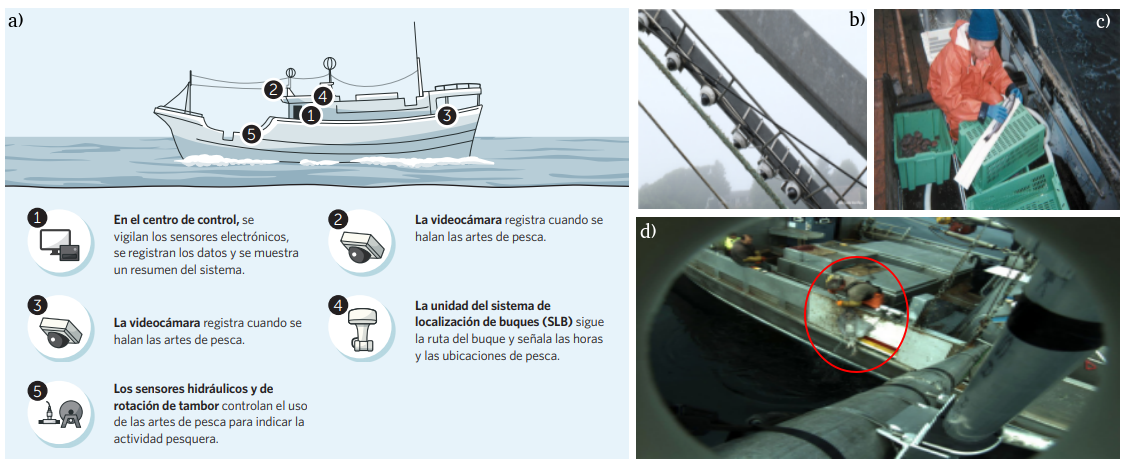
\includegraphics[width=1.\textwidth]{./Figuras/seguimiento_electronico.png}
\caption{ a) Sistema de Seguimiento Electrónico. b) Sistema de CCTV que apunta a redes de arrastre. c) Registro de especímenes por observadores calificados. d) Cámara captando descarte de especie protegida, probablemente no declarada.}
\label{fig:seguimiento_electronico}
\end{figure}

\vspace{25px}

\subsection{Marco de la propuesta}

INVAP S.E. es una empresa del Gobierno de Río Negro dedicada al diseño y construcción de sistemas tecnológicos complejos, con una trayectoria de cuatro décadas en el mercado nacional y tres en la escena internacional. La empresa define como su misión el desarrollo de tecnología de avanzada en diferentes campos de la industria, la ciencia y la investigación aplicada, creando “paquetes tecnológicos” de alto valor agregado tanto para satisfacer necesidades nacionales como para insertarse en mercados externos a través de la exportación.
Dentro del contexto de la búsqueda de nuevos negocios e incorporación de nuevas tecnologías, se realizan trabajos de investigación y prototipos, a menudo mediante convenios con universidades y otras organizaciones, ya sea en calidad de pasantías, prácticas profesionales, trabajos de carreras de grado y posgrado, u otros. Estos trabajos pueden eventualmente evolucionar y aprovecharse en un proyecto de mayor envergadura.
El proyecto que se describe es uno de estos casos y se integra en un desarrollo de mayor alcance: un sistema de monitoreo electrónico que utiliza cámaras de video y computadoras o dispositivos auxiliares para el control de la pesca. 

Existe un plan de incorporar gradualmente mayores niveles de automatismo y capacidades de reporte en tiempo real a este sistema. 
El principal cliente interesado es el Estado Argentino, y en particular la Subsecretaría de Pesca y Acuicultura perteneciente a la Secretaría de Agricultura, Ganadería y Pesca del Ministerio de Agricultura, Ganadería y Pesca. Si bien no son clientes directos, es también importante mencionar la participación del Consejo Federal Pesquero (https://cfp.gob.ar/) y de INIDEP(https://www.argentina.gob.ar/inidep), organismos involucrados en el seguimiento y regulación de la explotación del recurso y promotores de la modernización de los sistemas de monitoreo y seguimiento. También pueden ser potenciales usuarios centros de investigación o entes privados que lo utilicen para registro propio. El desarrollo y vinculación con instituciones se realiza por medio de INVAP S.E.

Como se mencionó, este trabajo es un subproducto de un proyecto de mayor envergadura. El desarrollo actual de INVAP S.E. tiene como objetivos posibilitar el registro de video y de la información de otros dispositivos (por ejemplo motores de las redes de arrastre) para su posterior análisis en tierra (dependiendo del caso puede ser hasta luego de 30 días en el mar). La segunda etapa del desarrollo es el procesamiento y envío del parte de pesca en tiempo real, y por último la automatización de algunas tareas de análisis. Este trabajo es un prototipo para esta última etapa. 

\subsection{Descripción del proyecto}

La distorsión de lente de pez que suelen tener las cámaras de vigilancia, las condiciones de iluminación variables (zonas de escaso contraste por la fuerte saturación de luces fluorescentes y otras casi sin iluminar) y la dificultad para detectar una estructura por la forma y disposición de las presas hacen que resulte difícil garantizar una correcta detección por un método automático.

La figura \ref{fig:ejemplos_escenas} muestra ejemplos de los tipos de escenas en las cuales se apunta a realizar la detección.

\begin{figure}[htpb]
\centering 
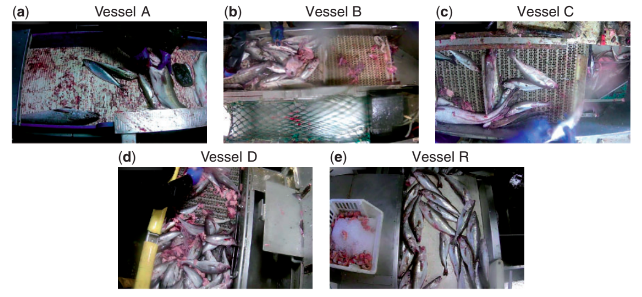
\includegraphics[width=1.\textwidth]{./Figuras/ejemplos_escenas.png}
\caption{Comparación de imágenes de cámaras en distintos buques. La orientación aleatoria de las presas y su mutua oclusión, y la difícil estructura de la escena presentan un desafío para los algoritmos de detección}
\label{fig:ejemplos_escenas}
\end{figure}

Aún así, la literatura consultada muestra que se pueden obtener resultados aceptables utilizando alguna variante de red convolucional (CNN, por sus siglas en inglés {\em Convolutional Neural Network}). 
Si bien no existe una restricción en la cantidad de neuronas mínima que deba tener una CNN, dado que
existe una relación entre la cantidad de neuronas o "profundidad" de una red y su capacidad de reconocimiento de patrones en escenas complejas, es usual que las CNN utilizadas para este tipo de tareas cuenten con múltiples capas, cada una destinada a extraer patrones de un nivel de abstracción creciente.
El inconveniente de las redes neuronales profundas es que requieren una gran cantidad de datos de entrenamiento, que en este caso (a diferencia de como ocurre en otros dominios, como el reconocimiento de personas, caras, vehículos, carteles, etc.) es difícil (o costoso) obtener.

La innovación de esta propuesta reside en la aplicación del estado del arte de estas técnicas a un dominio para el cual no existen productos o soluciones en el mercado.

La solución propuesta se compone de los siguientes bloques:

\begin{itemize}
\item Ingesta de Video: obtiene los cuadros de una cámara o un archivo de video y aplica una corrección de imagen para reducir las diferencias entre cámaras. Esta corrección puede incluir: contrarrestar distorsión de lente de pez, aplicar transformaciones de coordenadas cromáticas, ecualizar la imagen, entre otras.

\item Detección: este bloque recibe los cuadros de video procesados de la etapa anterior y por cada cuadro extrae las regiones de interés y la probabilidad de que exista alguna de las clases detectadas. Se utilizará el algoritmo YOLOv4 o variantes del mismo, dado que representa el estado del arte y es apto para procesamiento en tiempo real si se dispone del HW apropiado. A menudo la capacidad de detección de un objeto puede depender de su orientación, condiciones de oclusión, iluminación, etc. Es posible que un objeto que no sea fácilmente identificable en un cuadro de video, sí lo sea en otros cuadros de ese mismo video. Para este trabajo se propone usar un algoritmo de seguimiento que también representa el estado del arte, denominado DeepSORT. La salida de este algoritmo es una trayectoria de un objeto. Como etapa final, se propone un filtro para decidir si rechazar o no la detección y asociar un evento a esa trayectoria (por ejemplo, incrementar un contador de capturas, reportar un descarte, etc.).

\item Información de contexto (opcional): se puede utilizar información de localización del buque, fecha y hora, actividad de sistemas mecánicos y otros datos tanto para acompañar la salida del clasificador como para mejorarla, dado que hay especies que habitan determinados sectores o se capturan a determinada profundidade intervienen sistemas de captura específicos para un tipo de objetivo.

\item Registro y Generación de Reportes: la salida de la etapa anterior es registrada en una base de datos, para obtener trazabilidad de las capturas y descartes (horarios, tipos de capturas, cantidad de descartes, etc.). Para facilitar el consumo de esta información y permitir combinarla con otros servicios, se utilizará una base de datos con interfaz REST (por ejemplo InfluxDB).
\end{itemize}

La figura  \ref{fig:diagrama_bloques} muestra un diagrama de bloques de la solución propuesta.

\vspace{25px}

\begin{figure}[htpb]
\centering 
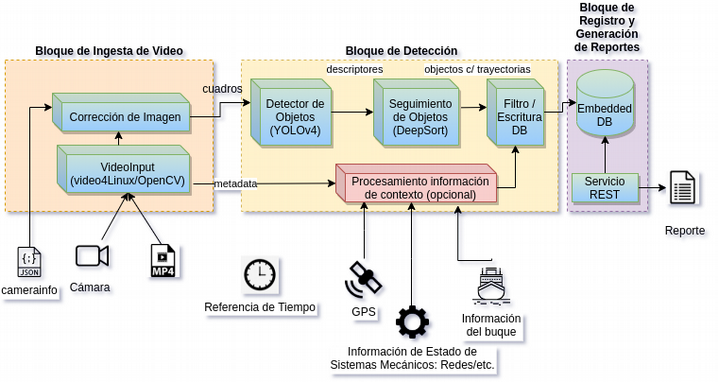
\includegraphics[width=1.\textwidth]{./Figuras/diagrama_bloques.png}
\caption{Diagrama en bloques del sistema}
\label{fig:diagrama_bloques}
\end{figure}

\vspace{25px}

\section{Identificación y análisis de los interesados}
\label{sec:interesados}

Dado que este proyecto es un subproducto de un desarrollo más completo de INVAP S.E. para el Estado, se considera como cliente a INVAP S.E.

\begin{table}[ht]
%\caption{Identificación de los interesados}
%\label{tab:interesados}
\begin{tabularx}{\linewidth}{@{}|l|X|X|l|@{}}
\hline
\rowcolor[HTML]{C0C0C0} 
Rol           & Nombre y Apellido & Organización 	& Puesto 	\\ \hline
Cliente       & \clientename      &\empclientename	& A confirmar     	\\ \hline
Responsable   & \authorname       & FIUBA        	& Alumno 	\\ \hline
Orientador    & \supname	      & \pertesupname 	& Director	Trabajo final \\ \hline
\end{tabularx}
\end{table}

\begin{itemize}
\item Usuario final: serán quienes actualmente realizan esta tarea de forma manual o nuevos operadores, pero aún no están designados.
\end{itemize}

\section{1. Propósito del proyecto}
\label{sec:proposito}

En línea con una estrategia de continua mejora e innovación, el propósito de este trabajo es incorporar al proyecto del sistema de seguimiento de pesca que está siendo actualmente desarrollado por INVAP S.E. un componente adicional para la automatización de las tareas de registro e inspección. 

\section{2. Alcance del proyecto}
\label{sec:alcance}

El presente proyecto contempla todo el software a desarrollar para el ciclo completo que se expuso en la figura \ref{fig:diagrama_bloques}, desde la adquisición de una imagen (utilizando los drivers o formato de publicación de las cámaras) hasta el reporte almacenado en las bases de datos. Hay una parte del hardware que ya está definida / o fuera del alcance (por ejemplo cámaras y algunas de las computadoras). También es parte de la solución recomendar un ambiente de ejecución.

Dado que el objetivo de este proyecto es estudiar la viabilidad técnica, dependiendo de los datos que puedan obtenerse de buques operativos o datos históricos, se seleccionará un subconjunto de especies a clasificar del total de las reportadas por INIDEP. 

Como cada especie tiene características especiales que permiten distinguirla, se realizará un estudio e ingeniería de características sobre esta selección para tratar de aprovecharlas en el algoritmo clasificador, incluyendo el arte de pesca y zonas de captura para obtenerlas -que determina el tipo de buque-, horario y temporada, parámetros operativos de los sistemas mecánicos de redes de arrastre (en caso que apliquen) y otros. Se utilizará como principal fuente de información la aportada por el cliente y será complementada con reportes e informes de INIDEP. 

\section{3. Supuestos del proyecto}
\label{sec:supuestos}

Para el desarrollo del presente proyecto se supone que:

\begin{itemize}
\item Se contará con los datos necesarios. Se recomienda un mínimo de 2000 ejemplos por cada clase de objeto a detectar. Si no pudiera alcanzarse este número, existen técnicas para compensar la falta de datos, pero puede verse penalizado el desempeño final del algoritmo y su capacidad de generalizar, siendo necesario un trabajo de ingeniería de {\em features } dependiendo de las características de las escenas en los que se utilizará.
\item Contando con datos de cantidad y calidad suficiente, los algoritmos de la familia YOLOv4 y DeepSORT serán aptos para resolver esta tarea con un desempeño igual o ligeramente superior al de un operador humano o de un mAP de 70\%.
\item Se contará con el HW disponible para desarrollo y ejecución del proyecto.
\item La ubicación y orientación de las cámaras puede variar dependiendo de la embarcación, pero una vez instaladas no serán modificadas. El proceso de configuración del SW se realiza sobre la configuración final de las cámaras.
\end{itemize}

\section{4. Requerimientos}
\label{sec:requerimientos}

\begin{enumerate}
\item Requerimientos generales
	\begin{enumerate}
	\item El sistema debe complementar una solución existente de hasta 4 cámaras de video para automatizar operaciones de conteo actualmente realizadas por operadores humanos.
	\end{enumerate}
\item Requerimientos funcionales
	\begin{enumerate}
	\item El sistema debe poder procesar video almacenado y en vivo en formato de color RGB y a resoluciones entre los 360p y 1080p. 
	\item El sistema debe detectar regiones de la imagen que contengan presas (pescados) en una escena con un porcentaje de confianza. El tipo de presas a detectar depende de cómo se haya configurado y entrenado el detector en cada caso.
	\item El sistema debe poder computar la trayectoria de un objeto detectado, con el propósito de asociar estas trayectorias a eventos. Por ejemplo, incrementar contadores, o indicar que una captura o descarte ingresó a una zona de la imagen.
	\item El sistema debe registrar todos los eventos de interés en una base de datos para su posterior utilización con fines estadísticos. Estos eventos se definen mediante la detección de un tipo de pieza en escena y que la misma ingrese, transite, o egrese de una región de la imagen previamente establecida (las cámaras siempre estarán en una posición fija). De este modo pueden definirse eventos como:
		\begin{itemize}
			\item Si una pieza está presente en una cinta transportadora.
			\item Si una pieza es arrojada por un lado del barco (indicando un descarte).
			\item El tiempo que permanece una pieza en un recipiente de la embarcación.
		\end{itemize}
	\end{enumerate}
\item Requerimientos de desempeño	
	\begin{enumerate}
	\item El procesamiento de video no puede estar por debajo de 1 cuadro procesado por segundo.
	\item El desempeño del detector debe ser equivalente o superior al de un operador humano medio, o en su defecto la detección debe cumplir como mínimo con un 70\% de mAP sobre un conjunto de datos de evaluación.
	\end{enumerate}
\item Requerimientos de interfaz
	\begin{enumerate}
	\item El sistema debe soportar por lo menos uno de los formatos de video estándar del mercado: RMTP, Video4Linux, etc.
	\item No se requiere una interfaz gráfica, pero sí la adhesión a protocolos estandar para poder acceder a la información. Ejemplos: REST,XML,JSON-RPC. 
	\item El sistema debe permitir indicar las regiones para cada cámara operativa en un archivo de configuración.
	\item Se debe proveer una guía de configuración y operación.
	\end{enumerate}	
\item Requerimientos de ambiente
	\begin{enumerate}
	\item Los componentes de procesamiento deberán ser servicios o microservicios y deben poder ejecutarse en un entorno Linux.
	\item La solución debe poder ejecutarse en una estación de trabajo, y con modificaciones menores poder correr, aunque sea con un desempeño degradado, en una plataforma embebida o {\em edge} (por ejemplo, la familia NVIDIA Xavier).
	\item La especificación exacta de la estación del trabajo es parte del trabajo a realizar (se proveerán tres recomendaciones de configuraciones de acuerdo a los productos disponibles en el mercado) pero debe contar con CPU, GPU, memoria RAM y almacenamiento acordes para la tarea. Una configuración posible es:
	\begin{itemize}
		\item CPU: Intel Xeon 2.60 GHz.
		\item RAM: 128GB  DDR4-2933.
		\item GPU: NVIDIA GeForce RTX 3090
		\item HD1: SSD 1TB
		\item HD2: SATA 10TB
	\end{itemize}
	\item Para simplificar el despliegue, es deseable pero no mandatorio el uso de docker u otra herramienta similar.
	\end{enumerate}		
\item Restricciones de diseño/implementación
	\begin{enumerate}
	\item El diseño debe ser modular y los componentes deben estar desacoplados, para poder realizar variaciones sobre la configuración según cada escenario.
	\item El código a desarrollar debe ser en Python o C/C++.
	\end{enumerate}	
\end{enumerate}

\section{Historias de usuarios (\textit{Product backlog})}
\label{sec:backlog}

Se identifican los siguientes roles:

\begin{itemize}
	\item Experto/analísta: conoce el dominio del problema y como mínimo cuenta con un manejo básico de herramientas de análisis de datos. Su función es confeccionar reportes a partir de los datos recopilados que alimentan decisiones estratégicas, como por ejemplo establecer cuotas de captura o reasignar zonas permitidas de explotación del recurso. Puede ser un científico del INIDEP.
	\item Administrador del Sistema ({\em SysAdmin}): es la persona que se responsabiliza de la instalación y configuración del SW y HW (no necesariamente desarrollador). Tiene conocimientos avanzados de redes, sistemas operativos (en especial Linux), administración de bases de datos, despliegue de aplicaciones basadas en contenedores o servicios, asignación de carga a procesadores, y otras habilidades afines. No necesariamente está familiarizado con el dominio del problema. Contando con la documentación adecuada realiza y mantiene instalaciones de SW en sistemas complejos como por ejemplo centros de operación de radares, del sector aeroespacial o nuclear. Es una persona de INVAP S.E. y conoce los procesos de desarrollo y normativas de calidad.
	\item Operador a bordo: es la persona que opera el sistema a bordo del buque, pero sin ser ésta su función principal. En este caso su responsabilidad consiste en verificar que el sistema se encuentra en estado nominal mediante algún indicador en pantalla o comando de consola y tomar alguna acción ante un problema: reiniciar un servicio de SW o aparato o modificar una configuración. 
	\item Desarrollador de SW con perfil IA: realiza cambios en el SW para extender su funcionalidad. Propone estrategias para modificar algoritmos existentes e incorporar nuevos y los implementa y pone a prueba. Sus tareas pueden incluir: reentrenar modelos para incorporar más objetivos a la clasificación, modificar y agregar componentes en las cadenas de procesamiento o diagnosticar fallas en un algoritmo. Tiene conocimientos de C/C++ y python y conoce el proceso de desarrollo de SW de la empresa.
\end{itemize}

Para estimar el puntaje de cada historia de usuario se consideran tres aspectos que caracterizan las tareas involucradas en alcanzar cada objetivo:

\begin{itemize}
	\item Esfuerzo o tiempo requerido.
	\item Complejidad.
	\item Riesgo.
\end{itemize}

A cada ítem se asigna un puntaje de 1 (bajo) a 5 (alto). El puntaje final es el número de Fibonacci más próximo a la suma de los puntajes parciales.

Es importante distinguir entre esfuerzo y complejidad. Por ejemplo, para asegurar un buen desempeño del algoritmo de detección es fundamental contar con datos de entrada de calidad, pero también con un modelo que haya sido configurado con los parámetros óptimos para esos datos de entrada. 

La recopilación, preprocesamiento, etiquetado y corrección manual de los datos es una tarea repetitiva, que insume tiempo, pero relativamente sencilla y de bajo riesgo.

En cambio, el diagnóstico y selección de parámetros de un modelo de red neuronal requiere un conocimiento profundo de la arquitectura y comportamiento de las unidades internas. Se nutre de ensayos cuya implementación es de pocas líneas de código, pero que deben diseñarse para evidenciar comportamientos de la red en escenarios específicos. Es una tarea compleja.

Para este proyecto se considera como máximo riesgo no poder cumplir con un desempeño mínimo en la tarea de detección, ya sea porque los datos son insuficientes, porque se excede la capacidad de cómputo estimada, o porque directamente no se puede dar con una configuración apta para resolver el problema.

Se considera a las tareas de preprocesamiento, organización e integración de componentes y documentación, extensivas en tiempo pero de bajo riesgo y complejidad. Esto es porque en INVAP S.E. se cuenta con experiencia en el desarrollo de sistemas de SW complejos con arquitecturas distribuidas.

Historia: definición de eventos

Como {\em experto/analista}, y habiendo participado de la ubicación y orientación de las cámaras a bordo, deseo poder definir regiones de la imagen para cada una de las cámaras y habilitar el registro de las piezas que ingresan a una región, las que salen de una región, y el tiempo que permanece una pieza en una región. 
\begin{itemize}
	\item Esfuerzo: bajo. Peso 2
	\item Complejidad: baja. Peso 2
	\item Riesgo: bajo. Peso 1
	\item Total: 5.
	\item Puntaje: 5.
\end{itemize}

Historia: consulta de datos

Como {\em experto/analista } deseo poder consultar todos los eventos registrados durante un intervalo de tiempo y obtener los resultados en un formato estándar como XML, CSV, JSON, API REST, u otro para que puedan ser tratados con otra herramienta específica, como por ejemplo python, R o Matlab. 
Estos resultados deben discriminar, como mínimo, fecha y hora y tipo de evento, para luego poder confeccionar estadísticas de actividad por momentos del día, total de capturas por tipo de pieza, total de descartes, cumplimiento de normas (permanencia máxima de una pieza en una cinta transportadora o recipiente), y otros.
\begin{itemize}
	\item Esfuerzo: bajo. Peso 1
	\item Complejidad: baja. Peso 1
	\item Riesgo: bajo. Peso 1
	\item Total: 3.
	\item Puntaje: 3.
\end{itemize}
	
Historia: automatización confiable
	
Como {\em experto/analista} deseo contar con información de alta confiabilidad, similar a la que brindaría un experto a bordo, pero libre de sesgos por otros intereses. Es decir, la cantidad de eventos que hayan ocurrido y no hayan sido detectados y registrados debe ser muy baja, y las piezas deben estar identificadas correctamente, o indicando una confianza baja si se trata de situaciones que también puedan ser difíciles de distinguir para un operador humano.
\begin{itemize}
	\item Esfuerzo: medio. Peso 3
	\item Complejidad: alta. Peso 5
	\item Riesgo: alto. Peso 5
	\item Total: 13.
	\item Puntaje: 13.
\end{itemize}

Historia: mantenimiento del sistema

Como {\em administrador del sistema}, deseo que el sistema sea desplegado en forma de servicios o contenedores (docker) para poder monitorearlos y asignarles los recursos correspondientes (procesador, RAM, cuota de disco). Además, deben poder ser configurables por medio de un archivo o línea de comando. Deben generar un log estándar para poder integrarse a un sistema de monitoreo.
	
\begin{itemize}
	\item Esfuerzo: alto. Peso 4
	\item Complejidad: baja. Peso 1
	\item Riesgo: bajo. Peso 1
	\item Total: 6.
	\item Puntaje: 5.
\end{itemize}

Historia: operación del sistema a bordo

Como {\em operador a bordo} deseo contar con un instructivo breve y conciso para iniciar el sistema, saber si está operativo, y realizar las tareas de mantenimiento (cambios de disco, verificación de conexiones, u otros.
	
\begin{itemize}
	\item Esfuerzo: bajo. Peso 1
	\item Complejidad: baja. Peso 1
	\item Riesgo: bajo. Peso 1
	\item Total: 3.
	\item Puntaje: 3.
\end{itemize}

Historia: desarrollo y mantenimiento del SW del sistema

Como {\em desarrollador de SW con perfil IA}, deseo contar con un ambiente de desarrollo y la documentación del código y los modelos implementados, así como la justificación para los parámetros elegidos. 
\begin{itemize}
	\item Esfuerzo: alto. Peso 4
	\item Complejidad: baja. Peso 2
	\item Riesgo: bajo. Peso 1
	\item Total: 7.
	\item Puntaje: 8.
\end{itemize}

Historia: desarrollo y evolución del sistema

Como {\em desarrollador de SW con perfil IA}, deseo que la solución esté implementado de manera modular, con componentes que cumplan funciones específicas y puedan recombinarse para formar otras cadenas de procesamiento para ensayar modos de operación con funcionalidades alternativas.
\begin{itemize}
	\item Esfuerzo: alto. Peso 4
	\item Complejidad: baja. Peso 2
	\item Riesgo: bajo. Peso 1
	\item Total: 7.
	\item Puntaje: 8.
\end{itemize}	

\section{5. Entregables principales del proyecto}
\label{sec:entregables}

\begin{itemize}
\item Documento de diseño.
\item Manual de usuario.
\item Código fuente.
\item Informe final.
\end{itemize}

\section{6. Desglose del trabajo en tareas}
\label{sec:wbs}

\begin{enumerate}
\item Relevamiento y capacitación
	\begin{enumerate}
		\item ID01. Lectura y relevamiento. Capacitación general. (40 hs)
	\end{enumerate}
\item Bloque de recepción de video.
	\begin{enumerate}
	\item ID02. Codificación (40 hs)
	\item ID03. Calibración y corrección (60 hs)
	\end{enumerate}
\item Bloque de detección
	\begin{enumerate}
	\item ID04. Desarrollo/entrenamiento de modelos (60 hs)
	\item ID05 Integración con DeepSORT (60 hs)
	\item ID06. Filtro final. (40 hs)
	\end{enumerate}
\item Bloque de registro y generación de reportes
	\begin{enumerate}
	\item ID07 Implementación (60hs)
	\end{enumerate}
\item Iteraciones de desarrollo y mejora de modelos / selección de HPs
	\begin{enumerate}
		\item ID08. Scripts de conversión de formatos (20 hs)
		\item ID09. Scripts de transformación de datos (20 hs)
		\item ID10. Gestión, organización y etiquetado de dataset (20 hs)
		\item ID11. Preparación de dataset (20 hs)
		\item ID12. Scripts de procesamiento de salidas/evaluación (30 hs)
		\item ID13. Scripts de particionamiento de datos (30 hs)
	\end{enumerate}	
\item Integración
	\begin{enumerate}
		\item ID14. Despliegue en PC (30 hs)
		\item ID15. Despliegue en Edge/NVIDIA Jetson/Xavier/similar (30 hs)
	\end{enumerate}	
\item Documentación
	\begin{enumerate}
	\item ID16. Documentación del producto (30 hs)
	\item ID17. Memorias (30 hs)
	\end{enumerate}		
\end{enumerate}

Cantidad total de horas: 620hs.

\section{7. Diagrama de Activity On Node}
\label{sec:AoN}

En la figura \ref{fig:aon}, se muestra el diagrama de {\em Activity On Node} con los tiempos indicados en horas. Se indica el camino crítico que comienza con la implementación del bloque de recepción de video (ID01). 

La capacidad de procesar video de entrada y una corrección básica de la imagen (aún cuando no se soporten todos los formatos o se haya integrado con la cámara final) permite iniciar la implementación y primeros ensayos con el detector de objetos (ID04), para el cual se puede también avanzar con datos provisorios hasta disponer de los datos finales.

Es suficiente contar con una implementación mínima que permita la adquisición de video y cuente con un bloque detector para comenzar a trabajar en el problema de seguimiento (ID05). Nuevamente, no es necesario disponer de los datos finales, de hecho hasta puede ser conveniente implementar el bloque de seguimiento con datos de un problema conocido, como por ejemplo el seguimiento de personas, para luego reentrenarlo con los datos del dominio de este problema.

Si bien es recomendable implementar los bloques de salida de la cadena de procesamiento (ID06) y de generación de reportes (ID07) una vez establecidas las interfaces de los bloques antecesores, es posible también avanzar con estas tareas, por ejemplo en la selección de la base de datos y comunicación entre servicios. Se pueden utilizar datos de prueba en reemplazo de los reales para proceder con la integración (ID14).

Dada la menor disponibilidad del setup edge y las dificultades adicionales de depuración en un ambiente embebido/edge (ID15), es recomendable primero contar con el modelo final implementado en PC. No obstante, si esto no fuera posible, también se puede avanzar con esta tarea si se dispone del HW e implementaciones de los bloques de la cadena con algún grado de madurez.

Se espera incorporar datos durante todo el desarrollo del proyecto, conforme se conozca en mayor detalle la disposición y orientación de las cámaras, características de la instalación (iluminación, disposición de redes, cinta transportadora y otros dispsositivos) así como del tipo de presas y movimientos asociados a su tratamiento. Es parte de la estrategia el mostrar prototipos funcionales para incentivar la colaboración para obtener estos datos, sujeta al interés en el proyecto por parte del cliente y los colaboradores.

Los datos obtenidos pueden ser de distintos proveedores y por lo tanto es factible que tengan algún grado de heterogeneidad en su formato y organización por sido adquiridos en circunstancias distintas a las de la solución final. Antes de su utilización posiblemente se requieran tareas de preprocesamiento y reorganización. Algunas pueden ser relativamente sencillas -como ajustar cantidad de cuadros por segundo, resolución, ecualización de la imagen- y otras más complejas como aplicar correcciones de perspectiva, seleccionar datos de interés de grandes volumenes sin clasificar, o hasta tener que realizar algún tipo de extracción/etiquetado cuya automatización no sea totalmente inmediata (o en el peor caso, inviable).

Estas tareas de preparación son parte de la naturaleza del desarrollo de los modelos de aprendizaje automático. Es un proceso caracterizado por ser de tipo iterativo, en el que se repite un ciclo en el que se preparan entradas para versiones preliminares de los modelos y a partir del análisis de las salidas obtenidas se decide una estrategia que puede incluir modificar el preprocesamiento de los datos de entrada, los parámetros de entrenamiento o realizar cambios en la arquitectura de los modelos.

Cada iteración permite profundizar en la interpretación del modelo y especificar mejor los datos de entrada requeridos. Las tareas ID08 a ID13 representan estas actividades.

Por ser un proyecto principalmente de SW con un único desarrollador, no existe ninguna tarea o componente en el que no pueda avanzarse aunque sea parcialmente, ni recurso cuya demora en estar disponible sea completamente bloqueante. 

Además del producto a desarrollar es de interés la documentación del proceso, pues existen otros campos en los que la empresa puede aplicar la misma solución técnica. Por este motivo cada tarea es acompañada de actividades de documentación semiformal (en formato de cuadernos Jupyter o instructivos que acompañan al código. Es habitual hacer disponible esta información en servidores internos de la empresa como {\em gitlab} o documentación {\em wiki} de la red interna. 

Parte de esta información será modificada para incorporarse en la documentación formal y en las memorias (ID16 e ID17), y es también por ello que estas actividades se planifican luego de haber finalizado la implementación.

\begin{figure}[htpb]
\centering 
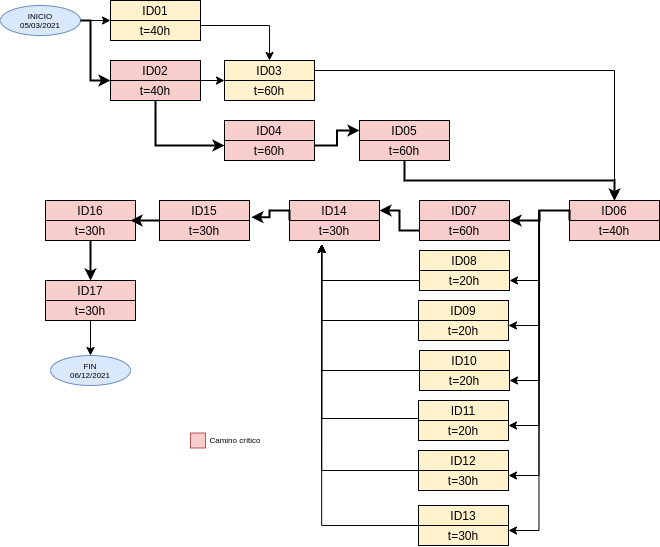
\includegraphics[width=1.\textwidth]{./Figuras/aon.png}
\caption{Diagrama de \textit{Activity On Node}}
\label{fig:aon}
\end{figure}

\section{8. Diagrama de Gantt}
\label{sec:gantt}

En la figura \ref{fig:gantt}, se muestra el diagrama de Gantt para la propuesta de trabajo. 

Por los motivos mencionados en el apartado anterior, se ha planificado la ejecución en paralelo de las tareas que pueden ejecutarse de manera concurrente y resulta difícil presuponer una secuencia con la información de que se dispone actualmente.

\begin{figure}[htpb]
\centering 
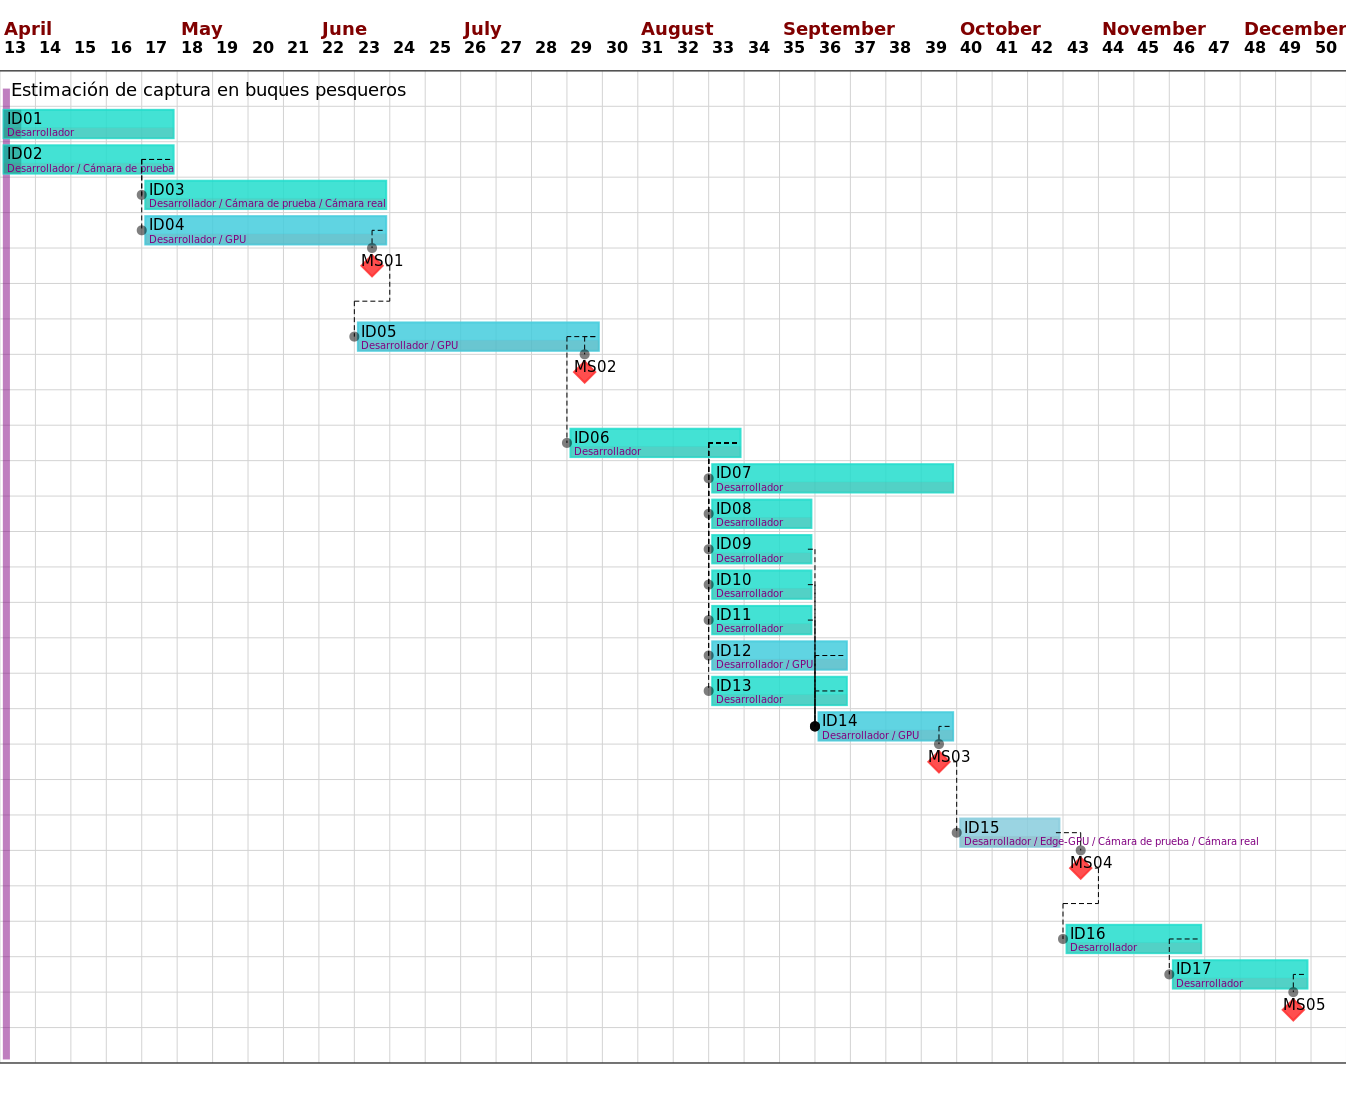
\includegraphics[width=1.\textwidth]{./Figuras/gantt.png}
\caption{Diagrama de \textit{Gantt}}
\label{fig:gantt}
\end{figure}

\section{9. Matriz de uso de recursos de materiales}
\label{sec:recursos}

Serán requeridos los siguientes materiales:

\begin{itemize}
	\item Cámara para pruebas: los ensayos con el algoritmo de seguimiento y bloque de adquisición y procesamiento de video pueden realizarse con una cámara económica de menores prestaciones a la de la instalación final. Puede ser una cámara HD tipo webcam con una tasa de 25 o más cuadros por segundo o similar. Es requisito que tenga soporte para Video4Linux y se integre sin mayores dificultades con OpenCV.
	\item Cámara final: modelo utilizado en la instalación final (o perteneciente a la misma familia). Será requerida para la calibración y selección de parámetros de corección de imagen en la implementación que se instalará al cliente. En caso de no tener acceso a la cámara, se pueden usar filmaciones para la parte de calibración y corrección.
	\item Ambiente de entrenamiento con GPU: el HW del que se dispone (de uso hogareño) resulta insuficiente para el entrenamiento de modelos de aprendizaje automático basados en redes profundas, por lo que esta tarea será ejecutada en un servidor dedicado que cuenta con mayores capacidades de cómputo y una o más GPUs dedicadas. Este servidor es compartido por otros usuarios y se accede por SSH, por lo que se utilizará únicamente para entrenar y evaluar modelos y no para desarrollo. La preparación de scripts se hará en otras PCs.
	\item Ambiente de ejecución con GPU: como el alcance del proyecto es de tipo prototipo, en caso de no disponer de otro ambiente de ejecución, se puede utilizar el mismo ambiente que para entrenamiento.
	\item Ambiente de ejecución {\em edge}: {\em Single Board Computer} (SBC) de la familia NVIDIA Jetson/Xavier o producto similar de otro fabricante. Se requiere para la versión del prototipo que realiza el procesamiento a bordo.
\end{itemize}

\begin{table}[htpb]
\label{tab:recursos}
\centering
\begin{tabularx}{\linewidth}{@{}|c|X|X|X|X|c|@{}}
\hline
\cellcolor[HTML]{C0C0C0} & \cellcolor[HTML]{C0C0C0} & \multicolumn{4}{c|}{\cellcolor[HTML]{C0C0C0}Recursos requeridos (horas)} \\ \cline{3-6} 
\multirow{-2}{*}{\cellcolor[HTML]{C0C0C0}\begin{tabular}[c]{@{}c@{}}Código\\ WBS\end{tabular}} & \multirow{-2}{*}{\cellcolor[HTML]{C0C0C0}\begin{tabular}[c]{@{}c@{}}Nombre \\ tarea\end{tabular}} & Cámara para pruebas & GPU & Cámara real & Setup EDGE \\ \hline
ID02 & Bloque de recepción de video. Codificación & 40 & 0 & 0 & 0  \\ \hline

ID03 & Bloque de recepción de video. Calibración y corrección.
     & 60 & 0 & 60 & 0  \\ \hline

ID04 & Bloque de detección. Desarrollo y entrenamiento.
     & 0 & 60 & 0 & 0   \\ \hline
     
ID05 & Bloque de detección. Integración con {\em DeepSORT}.
	 & 0 & 60 & 0 & 0  \\ \hline

ID12 & Iteraciones de desarrollo y mejora de modelos.
     & 0 & 30 & 0 & 0 \\ \hline

ID14 & Integración. Despliegue en PC.
     & 0 & 30 & 0 & 0 \\ \hline

ID15 & Integración. Despliegue en {\em edge}.
     & 30 & 0 & 30 & 30 \\ \hline

\end{tabularx}%
\end{table}

\section{10. Presupuesto detallado del proyecto}
\label{sec:presupuesto}

Se presenta un presupuesto para el desarrollo de un prototipo y suponiendo que el proyecto no se ejecuta en el contexto actual de relación dependencia de INVAP S.E. Esto se hace principalmente a modo de ejercicio teórico.

Se consideran como costos directos los materiales mínimos para tener un prototipo operativo en su version { \em Edge } y las horas de ingeniería y desarrollo.

Se consideran como costos indirectos la contratación de un espacio de trabajo y de horas de cómputo, tomando como referencia una experiencia personal de entrenamiento en Google Cloud de un modelo sencillo de detección de objetos incluyendo el almacenamiento de los datos, con un costo de U\$S 67. Se considera un promedio de U\$S 250 por contratación de servicios en la nube para preparación de datos y entrenamiento. Se ha asignado un monto menor del presupuesto para insumos y asesoramiento legal.

\begin{table}[htpb]
\centering
\begin{tabularx}{\linewidth}{@{}|X|c|r|r|@{}}
\hline
\rowcolor[HTML]{C0C0C0} 
\multicolumn{4}{|c|}{\cellcolor[HTML]{C0C0C0}COSTOS DIRECTOS} \\ \hline
\rowcolor[HTML]{C0C0C0} 
Descripción &
  \multicolumn{1}{c|}{\cellcolor[HTML]{C0C0C0}Cantidad} &
  \multicolumn{1}{c|}{\cellcolor[HTML]{C0C0C0}Valor unitario} &
  \multicolumn{1}{c|}{\cellcolor[HTML]{C0C0C0}Valor total} \\ \hline
NVIDIA Jetson AGX Xavier Developer Kit (*) (32GB) &
  \multicolumn{1}{c|}{1} &
  \multicolumn{1}{c|}{164.840,64	} &
  \multicolumn{1}{c|}{164.840,64	} \\ \hline
HIKVISION 4MPX PoE Outdoor Camera (*) &
  \multicolumn{1}{c|}{1} &
  \multicolumn{1}{c|}{22.920,00} &
  \multicolumn{1}{c|}{22.920,00} \\ \hline
Desarrollo/ingeniería (HH) &  
  \multicolumn{1}{c|}{620} &
  \multicolumn{1}{c|}{3.000,00} &
  \multicolumn{1}{c|}{1.860.000,00} \\ \hline
Varios. Chasis, fichas, conectores, etc. &  
  \multicolumn{1}{c|}{1} &
  \multicolumn{1}{c|}{30.000,00} &
  \multicolumn{1}{c|}{30.000,00} \\ \hline  
\multicolumn{3}{|c|}{SUBTOTAL} &
  \multicolumn{1}{c|}{2.057.760,64} \\ \hline
\rowcolor[HTML]{C0C0C0} 
\multicolumn{4}{|c|}{\cellcolor[HTML]{C0C0C0}COSTOS INDIRECTOS} \\ \hline
\rowcolor[HTML]{C0C0C0} 
Descripción &
  \multicolumn{1}{c|}{\cellcolor[HTML]{C0C0C0}Cantidad} &
  \multicolumn{1}{c|}{\cellcolor[HTML]{C0C0C0}Valor unitario} &
  \multicolumn{1}{c|}{\cellcolor[HTML]{C0C0C0}Valor total} \\ \hline
\multicolumn{1}{|l|}{Alquiler oficina c/ servicios (mensual)	} &
8  & 45.000,0  & 360.000,0 \\ \hline
\multicolumn{1}{|l|}{Servicio de cómputo (mensual)	} &
8  & 64.176,0.0  & 513.408,0 \\ \hline
\multicolumn{1}{|l|}{Insumos} &
8  & 5.000,0  & 24.000,0 \\ \hline
\multicolumn{1}{|l|}{Consultoría legal} &
2  & 14.000,0  & 28.000,0 \\ \hline
\multicolumn{3}{|c|}{SUBTOTAL} & 
  \multicolumn{1}{c|}{925.408,0} \\ \hline
\rowcolor[HTML]{C0C0C0}
\multicolumn{3}{|c|}{TOTAL} &
3.003.168,64  \\ \hline
\end{tabularx}%
\end{table}

Nota: los precios indicados con (*) fueron convertidos tomando el dólar a \$91 y considerando costos de importanción. Consultado: 5 de abril de 2021.


\section{11. Matriz de asignación de responsabilidades}
\label{sec:responsabilidades}

\begin{table}[htpb]
\centering
\resizebox{\textwidth}{!}{%
\begin{tabular}{|c|c|c|c|c|}
\hline
\rowcolor[HTML]{C0C0C0} 
\cellcolor[HTML]{C0C0C0} &
  \cellcolor[HTML]{C0C0C0} &
  \multicolumn{3}{c|}{\cellcolor[HTML]{C0C0C0}Roles del proyecto} \\ \cline{3-5} 
\rowcolor[HTML]{C0C0C0} 
\cellcolor[HTML]{C0C0C0} &
  \cellcolor[HTML]{C0C0C0} &
  Responsable &
  Orientador &
  Cliente \\ \cline{3-5} 
\rowcolor[HTML]{C0C0C0} 
\multirow{-3}{*}{\cellcolor[HTML]{C0C0C0}\begin{tabular}[c]{@{}c@{}}Código\\ WBS\end{tabular}} &
  \multirow{-3}{*}{\cellcolor[HTML]{C0C0C0}Nombre de la tarea} &
  N.E. Horro &
  F.R. Rojo &
  J.O. Lugo \\ \hline
ID01 & Lectura y relevamiento. Capacitación general.           & P &     C & - \\ \hline
ID02 & Bloque de recepción de video. Codificación.             & P &     C & - \\ \hline
ID03 & Bloque de recepción de video. Calibración y corrección. & P &     C & - \\ \hline
ID04 & Bloque de detección. Desarrollo/entrenamiento.          & P &   C/A & - \\ \hline
ID05 & Bloque de detección. Integración con DeepSORT.          & P &   C/A & - \\ \hline
ID06 & Bloque de detección.Filtro final.                       & P &   C/A & - \\ \hline
ID07 & Bloque de registro y generación de reportes.            & P &   C/A & I \\ \hline
ID08 & Desarrolllo iterativo. 
       Scripts de conversión de formatos.
     & P &   C/A & - \\ \hline
ID09 & Desarrolllo iterativo.
       Scripts de transformación de datos.
     & P &   C/A & - \\ \hline
ID10 & Desarrolllo iterativo.
       Gestión, organización y etiquetado de dataset.
     & P &   C/A & S \\ \hline
ID11 & Desarrolllo iterativo.
       Preparación de dataset.
     & P &     C & S \\ \hline
ID12 & Desarrolllo iterativo.
       Scripts de procesamiento de salidas/evaluación.
     & P &   C/A & - \\ \hline
ID13 & Desarrolllo iterativo.
       Scripts de particionamiento de datos.
     & P &   C/A & - \\ \hline
ID14 & Integración. Despliegue en PC.                 
     & P &     C & A \\ \hline
ID15 & Integración. Despliegue en Edge.               
     & P &     C & A \\ \hline
ID16 & Documentación del producto.                    
     & P &   C/A & A \\ \hline
ID17 & Documentación. Memorias.                       
     & P &   C/A & - \\ \hline 
 
 
\end{tabular}%
}
\end{table}

{\footnotesize
Referencias:
\begin{itemize}
	\item P = Responsabilidad Primaria
	\item S = Responsabilidad Secundaria
	\item A = Aprobación
	\item I = Informado
	\item C = Consultado
\end{itemize}
} %footnotesize

\section{12. Gestión de riesgos}
\label{sec:riesgos}

% --- BEGIN WIP -------------------------------------------------
Se identifican los siguientes riesgos para este proyecto. Se utilizará una escala de 1 a 10 para cuantificar la probabilidad de ocurrencia (10 es máxima probabilidad) y la severidad (10 es máxima severidad).

Riesgo 1. Datos insuficientes: no se consiguen datos de calidad en tiempo y forma. Los datos son insuficientes para entrenar el algoritmo, requieren más trabajo manual de preparación del planificado o están disponibles muy cerca de las fechas límite.
\begin{itemize}
	\item Severidad (S): 10. La calidad de los datos es quizás el aspecto más importante en un problema de aprendizaje automático. Es muy difícil obtener buenos resultados si los datos son insuficientes, por lo que se considerará que este es el riesgo más severo del proyecto.
	\item Probabilidad de ocurrencia (O): 6. Las cámaras con las que se obtienen los datos de las embarcaciones deben importarse y la instalación y operación implica coordinar de recursos. No se tiene control sobre la prioridad que se dé a estas actividades. 
\end{itemize}

Riesgo 2. Bajo desempeño de los modelos: los resultados obtenidos por los algoritmos están por debajo de los esperados.
\begin{itemize}
	\item Severidad (S): 10. Si el reporte generado por el algoritmo está muy por debajo de lo esperado y no se puede confiar en las detecciones, la propuesta de utilizar IA se torna inviable.
	\item Probabilidad de ocurrencia (O): 4. Los algoritmos han sido ensayados en otros escenarios y se están utilizando en otros campos de la industria con resultados aceptables, pero no deja de ser un área novedosa sobre la cual no se tiene experiencia suficiente.
\end{itemize}

Riesgo 3. Costo excesivo de desarrollo: los análisis y evolución muestran resultados favorables, pero se requiere más esfuerzo del previsto. La complejidad de ambientes y herramientas, tiempos de entrenamiento, diagnóstico de fallas insumen mayores horas de las planificadas y retrasan y consumen horas asignadas a otras tareas.
\begin{itemize}
	\item Severidad (S): 5. Si bien afecta la planificación original y los hitos comprometidos, puede no ser fatal para el resultado del proyecto.
	\item Probabilidad de ocurrencia (O): 9. Las herramientas y técnicas utilizadas tienen una complejidad considerable y el esfuerzo dedicado a resolver obstáculos puede extenderse.
\end{itemize}

Riesgo 4. No se dispone de recursos. Por factores fuera de control (por ejemplo, cambio de prioridades) se asignan los recursos a otras funciones (HW o dedicación de mano de obra).
\begin{itemize}
	\item Severidad (S): 6. Afecta la planificación original, pero pueden renegociarce los plazos y alcance para adecuarlo a los recursos disponibles.
	\item Probabilidad de ocurrencia (O): 3. No hay eventos que comprometan los recursos del proyecto identificados hasta el momento.
\end{itemize}

Riesgo 5. No se interpretaron correctamente las necesidades del cliente. Las funciones implementadas no son valoradas y en cambio, se esperan otras funciones que no están dentro del alcance.
\begin{itemize}
	\item Severidad (S): 2. Es normal que esto ocurra y tenga que haber modificaciones en las funciones. Si son cambios de impacto moderado y avisados con tiempo, pueden negociarse en los hitos y alcance y replanificarse las tareas.
	\item Probabilidad de ocurrencia (O): 9. Es habitual en el desarrollo de SW, y los métodos ágiles incluso lo fomentan y proponen estrategias para manejarlo.
\end{itemize}

Tabla de gestión de riesgos:

\begin{table}[htpb]
\centering
\begin{tabularx}{\linewidth}{@{}|X|c|c|c|c|c|c|@{}}
\hline
\rowcolor[HTML]{C0C0C0} 
Riesgo                        & S  &  O & RPN & S* & O* & RPN* \\ \hline
1. Datos insuficientes. 	  & 10 &  6 & 60  & 5  & 6  & 30   \\ \hline
2. Bajo desempeño de modelos. & 10 &  4 & 40  & 5  & 2  & 10   \\ \hline
3. Costo excesivo. 			  &  5 &  9 & 45  & 2  & 4  & 8    \\ \hline
4. Falta de recursos. 		  &  6 &  3 & 18  & -  & -  & -    \\ \hline
5. Alcance errado. 			  &  2 &  9 & 18  & -  & -  & -    \\ \hline
\end{tabularx}%
\end{table}

Se tomarán medidas de mitigación en los riesgos cuyos números de RPN sean mayores a 18.

Nota: los valores marcados con (*) en la tabla corresponden luego de haber aplicado la
mitigación.

Plan de mitigación de los riesgos que originalmente excedían el RPN máximo establecido:

Riesgo 1. Datos insuficientes: plan de mitigación. Lograr el mayor avance posible con datos suplementarios. Existen fuentes de datos públicos que si bien no son para las especies del mar argentino, aplican para un problema muy similar \footnote{Por ejemplo: https://www.kaggle.com/c/the-nature-conservancy-fisheries-monitoring y https://www.fishnet.ai/)}.
\begin{itemize}
	\item Nueva asignación de S y O: 30.
	\subitem Severidad (S): 5. Obtener un modelo que no se ajuste a los requerimientos específicos del cliente contradice un poco el espíritu de la solución, pero no invalida la solución técnicamente, y es posible acercarse al objetivo original con técnicas como transfer learning o one-shot learning con muy pocos datos de entrenamiento. De todos modos, sigue siendo un escenario poco favorable.
	\subitem Probabilidad de ocurrencia (O): 6. La probabilidad de ocurrencia no se modifica por el plan de mitigación elegido.
\end{itemize}

Riesgo 2. Bajo desempeño de modelos: plan de mitigación. Profundizar en las arquitecturas y fundamentos matemáticos de cada modelo para poder hacer ajustes y correcciones. Usar otros trabajos como referencia para incorporar mejoras. 
\begin{itemize}
	\item Nueva asignación de S y O: 10.
	\subitem Severidad (S): 5. realizar modificaciones sobre arquitecturas que conocidas penaliza la simplicidad de la solución e implica un esfuerzo adicional (puede ser más difícil convertir formatos y usar herramientas estándar, por ejemplo), pero compromete en menor grado los objetivos principales.
	\subitem Probabilidad de ocurrencia (O):2. Una buena comprensión de los algoritmos permite diagnosticar problemas y encontrar estrategias para solventarlos.
\end{itemize}

Riesgo 3. Costo excesivo: plan de mitigación. Renegociar el alcance y plazos de entrega. Procurar capitalizar esfuerzos de proyectos similares ({\em know-how} o reutilizar componentes) o con aspectos en común.
\begin{itemize}
	\item Nueva asignación de S y O: 8.
	\subitem Severidad (S): 2. Es posible recortar el alcance de componentes o aspectos no críticos y no comprometer los objetivos principales.
	\subitem Probabilidad de ocurrencia (O): 4. Un buen relevamiento previo a la ejecución de cada tarea puede mejorar la eficiencia.
\end{itemize}

\section{13. Gestión de la calidad}
\label{sec:calidad}

\begin{itemize}  % Inicio de lista de reqs.

% REQ
\item Req \#1: El sistema debe complementar una solución existente de hasta 4 cámaras de video para automatizar operaciones de inspección y conteo actualmente realizadas por operadores humanos.

Verificación y validación:
\subitem Verificación: realizar una configuración para la cantidad máxima de cámaras disponibles (hasta 4) y ejecutar el SW. Si no es posible generar eventos o acceder a las cámaras, se pueden utilizar grabaciones de las mismas, pero deben ser procesadas en paralelo. Se deben observar salidas independientes para cada cámara (eventos).
\subitem Método de validación: inspección.

% REQ
\item Req \#2: El sistema debe poder procesar video almacenado y en vivo en formato de color RGB y a resoluciones entre los 360p y 1080p. 

Verificación y validación:
\subitem Verificación: configurar cada cámara en distintos valores del intervalo soportado y verificar que el sistema detecta eventos (es admisible que en bajas resoluciones haya una disminución de la capacidad de detección, dependiendo de características de la escena).
\subitem Método de validación: inspección.

% REQ
\item Req \#3: El sistema debe detectar regiones de la imagen que contengan presas (pescados) en una escena con un porcentaje de confianza. El tipo de presas a detectar depende de cómo se haya configurado y entrenado el detector en cada caso.

Verificación y validación:
\subitem Verificación: comparar los resultados del sistema contra resultados generados manualmente por operadores. Nota: para esto se utiliza un video anotado, es decir, se acompaña al video con uno o más archivos de texto que contienen las detecciones esperadas en cada cuadro (puede utilizarse interpolación).
\subitem Validación: ensayo cuantitativo.

% REQ
\item Req \#4: El sistema debe poder computar la trayectoria de un objeto detectado, con el propósito de asociar estas trayectorias a eventos. Por ejemplo, incrementar contadores, o indicar que una captura o descarte ingresó a una zona de la imagen.

Verificación y validación:
\subitem Verificación: comparar los resultados del sistema contra resultados generados manualmente por operadores. Nota: al igual que en el caso anterior, se utiliza un video anotado.
\subitem Validación: ensayo cuantitativo.

% REQ
\item Req \#5: El sistema debe registrar todos los eventos de interés en una base de datos para su posterior utilización con fines estadísticos. Estos eventos se definen mediante la detección de un tipo de pieza en escena y que la misma ingrese, transite, o egrese de una región de la imagen previamente establecida (las cámaras siempre estarán en una posición fija). De este modo pueden definirse eventos como:
			\subitem Si una pieza está presente en una cinta transportadora.
			\subitem Si una pieza es arrojada por un lado del barco (indicando un descarte).
			\subitem El tiempo que permanece una pieza en un recipiente de la embarcación.

Verificación y validación:
\subitem Verificación: generar casos de prueba para distintos escenarios (videos en los que se cumpla alguno de estos eventos).
\subitem Validación: ensayo cuantitativo.

% REQ
\item Req \#6: El procesamiento de video no puede estar por debajo de 1 cuadro procesado por segundo.

Verificación y validación:
\subitem Verificación: medir el tiempo de inicio y término de procesamiento para un video de duración conocida.
\subitem Validación: ensayo cuantitativo.

% REQ
\item Req \#7: El desempeño del detector debe ser equivalente o superior al de un operador humano medio, o en su defecto la detección debe cumplir como mínimo con un 70\% de mAP sobre un conjunto de datos de evaluación \footnote{Si bien es reconocible la diferencia entre las piezas de captura y de descarte reflejadas en los partes de pesca y las que se estiman de acuerdo a otros estudios de INIDEP, no se dispone en este momento de una métrica que cuantifique el error entre la captura real y reportada por un operador.}.

Verificación y validación:
\subitem Verificación: seleccionar un conjunto de casos representativos. Cada caso es un video con anotaciones realizadas por un operador humano (eventos de interés). Comparar salida del sistema contra la de los operadores (cantidad de eventos acertados y errados para cada tipo, distinguiendo positivos, falsos positivos, negativos, y falsos negativos).
\subitem Validación: ensayo cuantitativo.

% REQ
\item Req \#8: El sistema debe soportar por lo menos uno de los formatos de video estándar del mercado: RMTP, Video4Linux, etc.

Verificación y validación:
\subitem Verificación: comprobar que el video se recibe correctamente.
\subitem Validación: inspección.

% REQ
\item Req \#9: No se requiere una interfaz gráfica, pero sí la adhesión a protocolos estandar para poder acceder a la información. Ejemplos: REST,XML,JSON-RPC. 

Verificación y validación:
\subitem Verificación: realizar un script de consulta de datos para casos de prueba establecidos (se pueden usar los de verificaciones anteriores).
\subitem Validación: ensayo cuantitativo.

% REQ
\item Req \#10: El sistema debe permitir indicar las regiones para cada cámara operativa en un archivo de configuración.

Verificación y validación:
\subitem Verificación: para un caso de prueba establecido, generar los archivos de configuración con las correspondientes regiones de interés y comprobar que se generan los eventos asociados (se pueden utilizar los scripts del ensayo anterior).
\subitem Validación: ensayo cuantitativo.

% REQ
\item Req \#11: Se debe proveer una guía de configuración y operación.

Verificación y validación:
\subitem Verificación: N/A.
\subitem Validación: inspección.

% REQ
\item Req \#12: Los componentes de procesamiento deberán ser servicios o microservicios y deben poder ejecutarse en un entorno Linux.

Verificación y validación:
\subitem Verificación: revisión de especialista.
\subitem Validación: inspección.

% REQ
\item Req \#13: La solución debe poder ejecutarse en una estación de trabajo, y con modificaciones menores poder correr, aunque sea con un desempeño degradado, en una plataforma embebida o {\em edge} (por ejemplo, la familia NVIDIA Xavier).

Verificación y validación:
\subitem Verificación: medir el desempeño en cuadros procesados por segundo a distintas resoluciones y cantidad de entradas habilitadas.
\subitem Validación: ensayo cuantitativo.

% REQ
\item Req \#14: El SW debe cumplir los requerimientos de desempeño en una configuración que cumpla con los requisitos mínimos de HW. Una configuración posible es:
	\begin{itemize}
		\item CPU: Intel Xeon 2.60 GHz.
		\item RAM: 128GB  DDR4-2933.
		\item GPU: NVIDIA GeForce RTX 3090
		\item HD1: SSD 1TB
		\item HD2: SATA 10TB
	\end{itemize}

Verificación y validación:
\subitem Verificación: medir el desempeño en cuadros procesados por segundo a distintas resoluciones y cantidad de entradas habilitadas.
\subitem Validación: ensayo cuantitativo.

% REQ
\item Req \#15:  El diseño debe ser modular y los componentes deben estar desacoplados, para poder realizar variaciones sobre la configuración según cada escenario.

\pagebreak

Verificación y validación:
\subitem Verificación: revisión de especialista.
\subitem Validación: inspección.

% REQ
\item Req \#15: El código a desarrollar debe ser en Python o C/C++.

Verificación y validación:
\subitem Verificación: revisión de especialista.
\subitem Validación: inspección.

\end{itemize} % Fin de lista de reqs.

% ================================================================ WIP

\section{14. Comunicación del proyecto}
\label{sec:comunicaciones}

El plan de comunicación del proyecto es el siguiente:

\begin{table}[htpb]
\centering
\begin{tabularx}{\linewidth}{@{}|X|C{2.4cm}|C{3cm}|C{1.8cm}|C{2cm}|C{2.1cm}|@{}}
\hline
\rowcolor[HTML]{C0C0C0} 
\multicolumn{6}{|c|}{\cellcolor[HTML]{C0C0C0}PLAN DE COMUNICACIÓN DEL PROYECTO}           \\ \hline
\rowcolor[HTML]{C0C0C0} 
¿Qué comunicar? & Audiencia & Propósito & Frecuencia & Método de comunicac.    & Responsable \\ \hline
Cambios de fase (ej: planificación a ejecución) &
\clientename, \supname                          &
Informar estado del proyecto, establecer prioridades para recursos            &
Espontáneo (cuando ocurra el evento)            &
email                                           &
\authorname                                     \\ \hline
Resultados de ensayos                           &
\supname                                        &
Evitar retrasos, consultar dudas, coordinar próximos pasos       &
Semanal                                         &
email, reportes                                 &
\authorname                                     \\ \hline
Objetivos parciales alcanzados                  &
\clientename, \supname                          &
Dar visibilidad de estado del proyecto          &
Semanal                                         &
email, reportes, video                                 &
\authorname                                     \\ \hline
Dificultades, desvíos, retrasos                  &
\clientename, \supname                          &
Mitigar impacto, buscar soluciones              &
Espontáneo (cuando ocurra el evento)            &
email                                           &
\authorname                                     \\ \hline
Solicitar recursos, notificar liberación de recursos &
\clientename, \supname                                &
Optimizar gestión de recursos                         &
Según necesidad (inicio y fin de tareas)              &
email                                                 &
\authorname                                      \\ \hline
Dar aviso de datos disponibles, actualizar alcance    &
\authorname, \supname                                &
Proveer entradas requeridas para desarrollo           &
Según necesidad (inicio y fin de tareas)              &
email                                                 &
\clientename                                      \\ \hline
% ¿Qué comunicar?
% Audiencia
% Propósito
% Frecuencia
% Método de comunicac.          
% Responsable      
                
\end{tabularx}
\end{table}

\section{15. Gestión de compras}
\label{sec:compras}

Para este proyecto se favorecerán proveedores nacionales, y en caso de no haberlos se eligirá el proveedor con menor tiempo de entrega y menor costo de envío.
Los materiales para ensamblado del prototipo (chasis, fichas, y conectores) pueden obtenerse de un proveedor nacional, mientras que en el caso de las cámaras y placa NVIDIA es probable que sean compras al exterior. En estos últimos casos existen muchas versiones del mismo producto con variaciones menores. Se buscará el que tenga mayor soporte en la comunidad de usuarios para facilitar la solución de problemas de compatiblidad e integración con otro SW.

\section{16. Seguimiento y control}
\label{sec:seguimiento}

Se indica para cada tarea del proyecto la frecuencia e indicadores propuestos.

Por ser un trabajo de SW / desarrollo de modelos de ML en el cual no existen componentes físicos se han considerado los siguientes indicadores de avance:

\begin{itemize}
	\item Líneas de Código (LDC). Es una métrica estándar en desarrollo de SW. Permite comparar el esfuerzo invertido en un componente comparándolo con componentes que realicen funciones en el mismo lenguaje de programación. No sólo es aplicable a lenguajes de programación, sino a cualquier archivo de texto. Los Sistemas de Control de Versiones (SVC) como GIT -que se utilizará en este proyecto- generan automáticamente reportes para esta y otras estadísticas, por lo que este indicador puede ser consultado a demanda del interesado sin intervención de los desarrolladores.
	\item Métricas. Si bien los modelos de aprendizaje automático se desarrollan en scripts que definen su arquitectura y parámetros, en general estos scripts suelen tener muy pocas LDC y es común reutilizarlos entre ensayos, por lo que las LDC no son un indicador útil en este caso. Tampoco es un buen indicador la complejidad de la red (cantidad de nodos, capas, coeficientes, etc.), pues por lo general se busca obtener el modelo más sencillo posible sin sacrificar desempeño. Aporta mayor valor conocer qué ensayos se realizaron, qué conclusiones se obtuvieron, y desde el punto de vista de los interesados en la solución, qué mejora se alcanzó en las métricas. Para esto se realizarán reportes en formato de cuadernos Jupyter. Se considera que un modelo de aprendizaje está progresando cuando se obtienen mejores métricas como resultado de haber hallado configuraciones de hiperparámetros óptimas y realizado modificaciones en la arquitectura. 
	\item Indicadores para tareas de organización y procesamiento. Hay dos motivos principales por los cuales se realizan estas tareas: cumplir con los requisitos de entrada de un algoritmo o implementación, y mejorar su desempeño. Por lo tanto se utilizan como indicadores para estas tareas la cantidad de ejemplos del dataset aptos para ser consumidos por los modelos, y se utilizan tests y métricas para evaluar el efecto de un tipo de procesamiento sobre el modelo final obtenido. También es de interés si se obtiene una disminución en el tiempo de entrenamiento como resultado de una mejor preparación de los datos.
	\item Indicadores para tareas de capacitación. La solución propuesta se apoya en dos algoritmos complejos: YOLOv4 y DeepSORT. Los avances en su estudio serán registrados en documentos técnicos informales (cuadernos Jupyter y apuntes) que luego serán formalizados en las memorias técnicas. En las reuniones con el director se tratarán temas específicos de cada algoritmo y como explotar sus capacidades.
	\item Cantidad de palabras/páginas/secciones será el indicador utilizado para documentación general que no pertenece a los casos anteriores.		
\end{itemize}

\begin{longtable}{|m{1cm}|m{3.5cm}|m{2.2cm}|m{2cm}|m{3cm}|m{1.5cm}|}
\hline
\rowcolor[HTML]{C0C0C0} 
\multicolumn{6}{|c|}{\cellcolor[HTML]{C0C0C0}SEGUIMIENTO DE AVANCE}                                                                       \\ \hline
\rowcolor[HTML]{C0C0C0} 
Tarea del WBS 			& Indicador de avance & Frecuencia de reporte & Resp. de seguimiento & Persona a ser informada & Método de comunic. \\ \hline
\endfirsthead

\hline
\rowcolor[HTML]{C0C0C0} 
\multicolumn{6}{c}{\cellcolor[HTML]{C0C0C0}SEGUIMIENTO DE AVANCE}                                                                       \\ \hline
\rowcolor[HTML]{C0C0C0} 
Tarea del WBS 			& Indicador de avance & Frecuencia de reporte & Resp. de seguimiento & Persona a ser informada & Método de comunic. \\ \hline
\endhead

\multicolumn{6}{c}{Continúa}
\endfoot

\endlastfoot

ID01 & Secciones técnicas escritas & Quincenal mientras dure la tarea& \authorname & \clientename, \supname & email / reunión \\ \hline 
ID02 & LDC & Quincenal mientras dure la tarea& \authorname / Automatizado con SCV & \clientename, \supname & SCV / email / reunión \\ \hline 
ID03 & LDC & Quincenal mientras dure la tarea& \authorname / Automatizado con SCV & \clientename, \supname & SCV / email / reunión \\ \hline 
ID04 & Tests / métricas & Quincenal mientras dure la tarea& \authorname / Automatizado con SCV & \clientename, \supname & SCV /email /reunión \\ \hline 
ID05 & Tests / métricas & Quincenal mientras dure la tarea& \authorname / Automatizado con SCV & \clientename, \supname & SCV / email / reunión \\ \hline 
ID06 & Tests / métricas & Quincenal mientras dure la tarea& \authorname / Automatizado con SCV & \clientename, \supname & SCV / email / reunión \\ \hline 
ID07 & LDC & Quincenal mientras dure la tarea& \authorname / Automatizado con SCV & \clientename, \supname & SCV / email / reunión \\ \hline 
ID08 & LDC, Cantidad de archivos convertidos & Quincenal mientras dure la tarea& \authorname / Automatizado con SCV & \clientename, \supname & SCV / email / reunión \\ \hline 
ID09 & Tests/métricas & Quincenal mientras dure la tarea& \authorname / Automatizado con SCV & \clientename, \supname & SCV / email / reunión \\ \hline 
ID10 & LDC, Cantidad de archivos preprocesados & Quincenal mientras dure la tarea& \authorname / Automatizado con SCV & \clientename, \supname & SCV / email / reunión \\ \hline 
ID11 & LDC, Operaciones realizadas & Quincenal mientras dure la tarea& \authorname / Automatizado con SCV & \clientename, \supname & SCV / email /reunión \\ \hline 
ID12 & LDC, Cantidad de reportes generados, tests / métricas & Quincenal mientras dure la tarea& \authorname / Automatizado con SCV & \clientename, \supname & SCV / email / reunión \\ \hline 
ID13 & LDC, Cantidad de reportes generados, tests / métricas & Quincenal mientras dure la tarea& \authorname / Automatizado con SCV & \clientename, \supname & SCV / email / reunión \\ \hline 
ID14 & LDC / cantidad de componentes integrados & Quincenal mientras dure la tarea& \authorname / Automatizado con SCV & \clientename, \supname & SCV / email / reunión \\ \hline 
ID15 & LDC / cantidad de componentes integrados & Quincenal mientras dure la tarea& \authorname / Automatizado con SCV & \clientename, \supname & SCV / email / reunión \\ \hline 
ID16 & cantidad de palabras/tamaño de archivos (de texto) & Quincenal mientras dure la tarea& \authorname / Automatizado con SCV & \clientename, \supname & SCV / email / reunión \\ \hline 
ID17 & cantidad de palabras/tamaño de archivos (de texto) & Quincenal mientras dure la tarea& \authorname / Automatizado con SCV & \clientename, \supname & SCV / email / reunión \\ \hline 
\end{longtable}

\section{17. Procesos de cierre}    
\label{sec:cierre}

Una vez entregado y aceptado el producto junto con su documentación correspondiente (incluyendo la documentación académica) se realizarán las siguientes actividades:

\begin{itemize}
\item Revisión del plan inicial propuesto para el proyecto y comparación con la ejecución. Se comparará el alcance propuesto del proyecto y específico para cada tarea, su esfuerzo estimado y el tiempo y esfuerzo reales ejecutados. También se evaluará si estuvieron disponibles los recursos en el tiempo es que estaba planificado. Esta actividad será realizada por el alumno y director.
\item Se identificarán las técnicas y procedimientos útiles e inútiles que se utilizaron, y los problemas que surgieron y cómo se solucionaron. 
Esta actividad será realizada por el alumno, director y cliente. Internamente la empresa tiene formas de registro en documentación de distintos niveles de formalidad: { \em wiki }, memorándum, o documento emitido. Se incluirá un resumen de esta información en las memorias.
\item Finalmente se organizará un acto de presentación y defensa del proyecto. Esta actividad será realizada por FIUBA.
\end{itemize}

\end{document}
